\documentclass[1p]{elsarticle_modified}
%\bibliographystyle{elsarticle-num}

%\usepackage[colorlinks]{hyperref}
%\usepackage{abbrmath_seonhwa} %\Abb, \Ascr, \Acal ,\Abf, \Afrak
\usepackage{amsfonts}
\usepackage{amssymb}
\usepackage{amsmath}
\usepackage{amsthm}
\usepackage{scalefnt}
\usepackage{amsbsy}
\usepackage{kotex}
\usepackage{caption}
\usepackage{subfig}
\usepackage{color}
\usepackage{graphicx}
\usepackage{xcolor} %% white, black, red, green, blue, cyan, magenta, yellow
\usepackage{float}
\usepackage{setspace}
\usepackage{hyperref}

\usepackage{tikz}
\usetikzlibrary{arrows}

\usepackage{multirow}
\usepackage{array} % fixed length table
\usepackage{hhline}

%%%%%%%%%%%%%%%%%%%%%
\makeatletter
\renewcommand*\env@matrix[1][\arraystretch]{%
	\edef\arraystretch{#1}%
	\hskip -\arraycolsep
	\let\@ifnextchar\new@ifnextchar
	\array{*\c@MaxMatrixCols c}}
\makeatother %https://tex.stackexchange.com/questions/14071/how-can-i-increase-the-line-spacing-in-a-matrix
%%%%%%%%%%%%%%%

\usepackage[normalem]{ulem}

\newcommand{\msout}[1]{\ifmmode\text{\sout{\ensuremath{#1}}}\else\sout{#1}\fi}
%SOURCE: \msout is \stkout macro in https://tex.stackexchange.com/questions/20609/strikeout-in-math-mode

\newcommand{\cancel}[1]{
	\ifmmode
	{\color{red}\msout{#1}}
	\else
	{\color{red}\sout{#1}}
	\fi
}

\newcommand{\add}[1]{
	{\color{blue}\uwave{#1}}
}

\newcommand{\replace}[2]{
	\ifmmode
	{\color{red}\msout{#1}}{\color{blue}\uwave{#2}}
	\else
	{\color{red}\sout{#1}}{\color{blue}\uwave{#2}}
	\fi
}

\newcommand{\Sol}{\mathcal{S}} %segment
\newcommand{\D}{D} %diagram
\newcommand{\A}{\mathcal{A}} %arc


%%%%%%%%%%%%%%%%%%%%%%%%%%%%%5 test

\def\sl{\operatorname{\textup{SL}}(2,\Cbb)}
\def\psl{\operatorname{\textup{PSL}}(2,\Cbb)}
\def\quan{\mkern 1mu \triangleright \mkern 1mu}

\theoremstyle{definition}
\newtheorem{thm}{Theorem}[section]
\newtheorem{prop}[thm]{Proposition}
\newtheorem{lem}[thm]{Lemma}
\newtheorem{ques}[thm]{Question}
\newtheorem{cor}[thm]{Corollary}
\newtheorem{defn}[thm]{Definition}
\newtheorem{exam}[thm]{Example}
\newtheorem{rmk}[thm]{Remark}
\newtheorem{alg}[thm]{Algorithm}

\newcommand{\I}{\sqrt{-1}}
\begin{document}

%\begin{frontmatter}
%
%\title{Boundary parabolic representations of knots up to 8 crossings}
%
%%% Group authors per affiliation:
%\author{Yunhi Cho} 
%\address{Department of Mathematics, University of Seoul, Seoul, Korea}
%\ead{yhcho@uos.ac.kr}
%
%
%\author{Seonhwa Kim} %\fnref{s_kim}}
%\address{Center for Geometry and Physics, Institute for Basic Science, Pohang, 37673, Korea}
%\ead{ryeona17@ibs.re.kr}
%
%\author{Hyuk Kim}
%\address{Department of Mathematical Sciences, Seoul National University, Seoul 08826, Korea}
%\ead{hyukkim@snu.ac.kr}
%
%\author{Seokbeom Yoon}
%\address{Department of Mathematical Sciences, Seoul National University, Seoul, 08826,  Korea}
%\ead{sbyoon15@snu.ac.kr}
%
%\begin{abstract}
%We find all boundary parabolic representation of knots up to 8 crossings.
%
%\end{abstract}
%\begin{keyword}
%    \MSC[2010] 57M25 
%\end{keyword}
%
%\end{frontmatter}

%\linenumbers
%\tableofcontents
%
\newcommand\colored[1]{\textcolor{white}{\rule[-0.35ex]{0.8em}{1.4ex}}\kern-0.8em\color{red} #1}%
%\newcommand\colored[1]{\textcolor{white}{ #1}\kern-2.17ex	\textcolor{white}{ #1}\kern-1.81ex	\textcolor{white}{ #1}\kern-2.15ex\color{red}#1	}

{\Large $\underline{11n_{99}~(K11n_{99})}$}

\setlength{\tabcolsep}{10pt}
\renewcommand{\arraystretch}{1.6}
\vspace{1cm}\begin{tabular}{m{100pt}>{\centering\arraybackslash}m{274pt}}
\multirow{5}{120pt}{
	\centering
	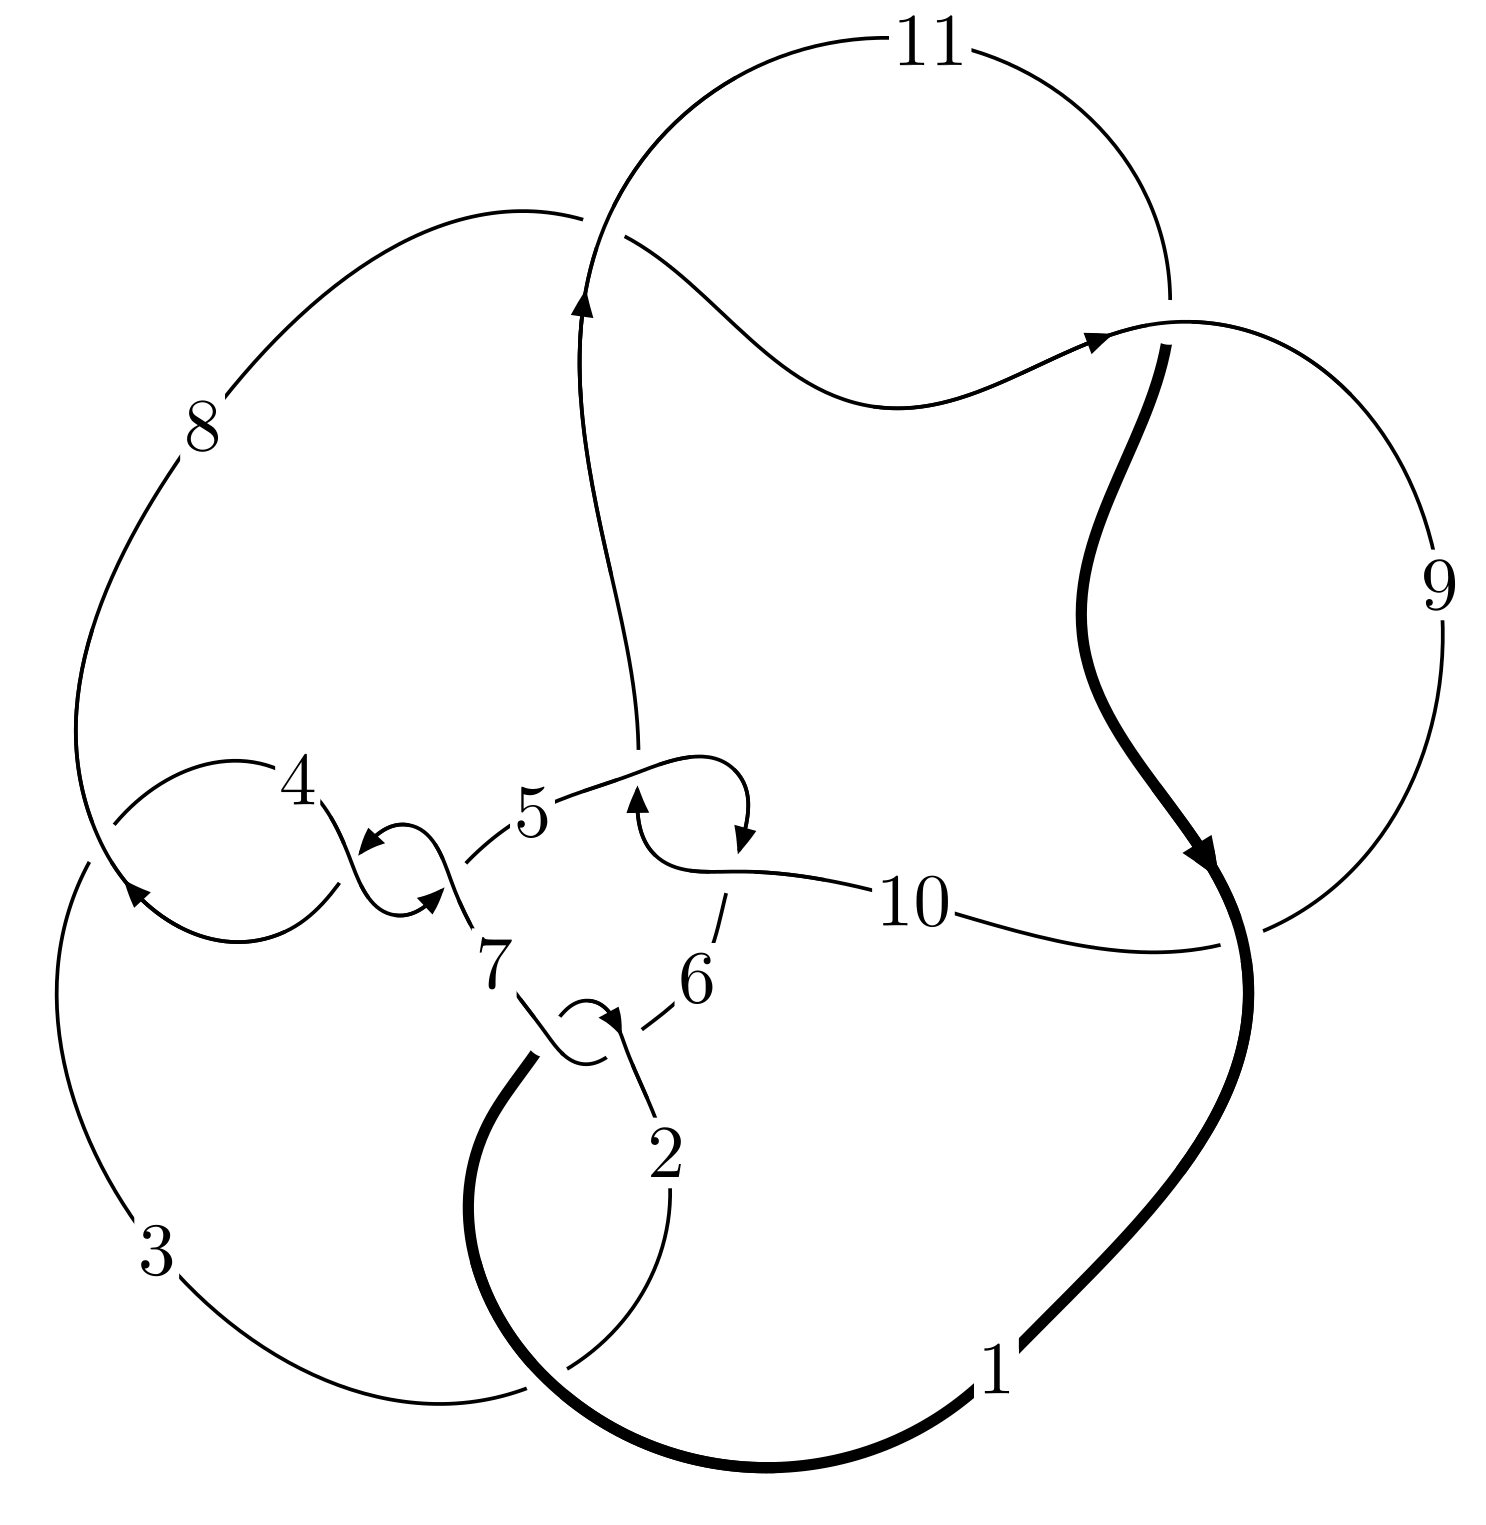
\includegraphics[width=112pt]{../../../GIT/diagram.site/Diagrams/png/715_11n_99.png}\\
\ \ \ A knot diagram\footnotemark}&
\allowdisplaybreaks
\textbf{Linearized knot diagam} \\
\cline{2-2}
 &
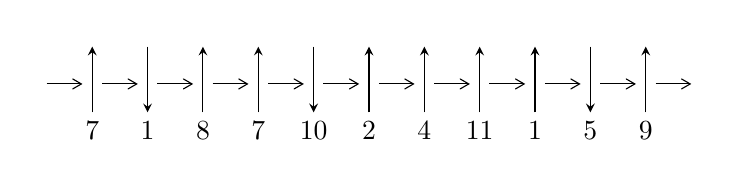
\begin{tikzpicture}[x=20pt, y=17pt]
	% nodes
	\node (C0) at (0, 0) {};
	\node (C1) at (1, 0) {};
	\node (C1U) at (1, +1) {};
	\node (C1D) at (1, -1) {7};

	\node (C2) at (2, 0) {};
	\node (C2U) at (2, +1) {};
	\node (C2D) at (2, -1) {1};

	\node (C3) at (3, 0) {};
	\node (C3U) at (3, +1) {};
	\node (C3D) at (3, -1) {8};

	\node (C4) at (4, 0) {};
	\node (C4U) at (4, +1) {};
	\node (C4D) at (4, -1) {7};

	\node (C5) at (5, 0) {};
	\node (C5U) at (5, +1) {};
	\node (C5D) at (5, -1) {10};

	\node (C6) at (6, 0) {};
	\node (C6U) at (6, +1) {};
	\node (C6D) at (6, -1) {2};

	\node (C7) at (7, 0) {};
	\node (C7U) at (7, +1) {};
	\node (C7D) at (7, -1) {4};

	\node (C8) at (8, 0) {};
	\node (C8U) at (8, +1) {};
	\node (C8D) at (8, -1) {11};

	\node (C9) at (9, 0) {};
	\node (C9U) at (9, +1) {};
	\node (C9D) at (9, -1) {1};

	\node (C10) at (10, 0) {};
	\node (C10U) at (10, +1) {};
	\node (C10D) at (10, -1) {5};

	\node (C11) at (11, 0) {};
	\node (C11U) at (11, +1) {};
	\node (C11D) at (11, -1) {9};
	\node (C12) at (12, 0) {};

	% arrows
	\draw[->,>={angle 60}]
	(C0) edge (C1) (C1) edge (C2) (C2) edge (C3) (C3) edge (C4) (C4) edge (C5) (C5) edge (C6) (C6) edge (C7) (C7) edge (C8) (C8) edge (C9) (C9) edge (C10) (C10) edge (C11) (C11) edge (C12) ;	\draw[->,>=stealth]
	(C1D) edge (C1U) (C2U) edge (C2D) (C3D) edge (C3U) (C4D) edge (C4U) (C5U) edge (C5D) (C6D) edge (C6U) (C7D) edge (C7U) (C8D) edge (C8U) (C9D) edge (C9U) (C10U) edge (C10D) (C11D) edge (C11U) ;
	\end{tikzpicture} \\
\hhline{~~} \\& 
\textbf{Solving Sequence} \\ \cline{2-2} 
 &
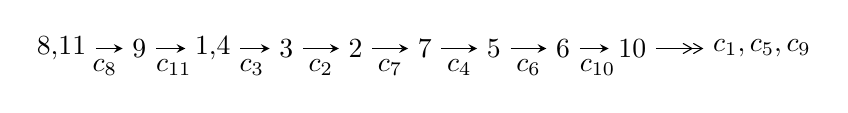
\begin{tikzpicture}[x=25pt, y=7pt]
	% node
	\node (A0) at (-1/8, 0) {8,11};
	\node (A1) at (1, 0) {9};
	\node (A2) at (33/16, 0) {1,4};
	\node (A3) at (25/8, 0) {3};
	\node (A4) at (33/8, 0) {2};
	\node (A5) at (41/8, 0) {7};
	\node (A6) at (49/8, 0) {5};
	\node (A7) at (57/8, 0) {6};
	\node (A8) at (65/8, 0) {10};
	\node (C1) at (1/2, -1) {$c_{8}$};
	\node (C2) at (3/2, -1) {$c_{11}$};
	\node (C3) at (21/8, -1) {$c_{3}$};
	\node (C4) at (29/8, -1) {$c_{2}$};
	\node (C5) at (37/8, -1) {$c_{7}$};
	\node (C6) at (45/8, -1) {$c_{4}$};
	\node (C7) at (53/8, -1) {$c_{6}$};
	\node (C8) at (61/8, -1) {$c_{10}$};
	\node (A9) at (10, 0) {$c_{1},c_{5},c_{9}$};

	% edge
	\draw[->,>=stealth]	
	(A0) edge (A1) (A1) edge (A2) (A2) edge (A3) (A3) edge (A4) (A4) edge (A5) (A5) edge (A6) (A6) edge (A7) (A7) edge (A8) ;
	\draw[->>,>={angle 60}]	
	(A8) edge (A9);
\end{tikzpicture} \\ 

\end{tabular} \\

\footnotetext{
The image of knot diagram is generated by the software ``\textbf{Draw programme}" developed by Andrew Bartholomew(\url{http://www.layer8.co.uk/maths/draw/index.htm\#Running-draw}), where we modified some parts for our purpose(\url{https://github.com/CATsTAILs/LinksPainter}).
}\phantom \\ \newline 
\centering \textbf{Ideals for irreducible components\footnotemark of $X_{\text{par}}$} 
 
\begin{align*}
I^u_{1}&=\langle 
-1338 u^{11}-2403 u^{10}+\cdots+24722 b+1642,\;-2813 u^{11}-3694 u^{10}+\cdots+49444 a-23561,\\
\phantom{I^u_{1}}&\phantom{= \langle  }u^{12}-2 u^{11}-3 u^{10}+7 u^9+3 u^8-10 u^7+12 u^6-17 u^5-14 u^4+34 u^3+2 u^2-7 u-4\rangle \\
I^u_{2}&=\langle 
u^5- u^4+u^2 a- u^3+2 u^2+b- a-1,\;- u^5+2 u^3 a+2 u^4-2 u^2 a+a^2- a u-2 u^2+2 a+2 u-1,\\
\phantom{I^u_{2}}&\phantom{= \langle  }u^6- u^5- u^4+2 u^3- u+1\rangle \\
I^u_{3}&=\langle 
- a u+b- a+1,\;a^2+2 a u-4 a-6 u+10,\;u^2- u-1\rangle \\
I^u_{4}&=\langle 
b-1,\;2 a+1,\;u+1\rangle \\
\\
\end{align*}
\raggedright * 4 irreducible components of $\dim_{\mathbb{C}}=0$, with total 29 representations.\\
\footnotetext{All coefficients of polynomials are rational numbers. But the coefficients are sometimes approximated in decimal forms when there is not enough margin.}
\newpage
\renewcommand{\arraystretch}{1}
\centering \section*{I. $I^u_{1}= \langle -1338 u^{11}-2403 u^{10}+\cdots+24722 b+1642,\;-2813 u^{11}-3694 u^{10}+\cdots+49444 a-23561,\;u^{12}-2 u^{11}+\cdots-7 u-4 \rangle$}
\flushleft \textbf{(i) Arc colorings}\\
\begin{tabular}{m{7pt} m{180pt} m{7pt} m{180pt} }
\flushright $a_{8}=$&$\begin{pmatrix}1\\0\end{pmatrix}$ \\
\flushright $a_{11}=$&$\begin{pmatrix}0\\u\end{pmatrix}$ \\
\flushright $a_{9}=$&$\begin{pmatrix}1\\- u^2\end{pmatrix}$ \\
\flushright $a_{1}=$&$\begin{pmatrix}u\\- u^3+u\end{pmatrix}$ \\
\flushright $a_{4}=$&$\begin{pmatrix}0.0568926 u^{11}+0.0747108 u^{10}+\cdots+2.87250 u+0.476519\\0.0541218 u^{11}+0.0972009 u^{10}+\cdots+0.203098 u-0.0664186\end{pmatrix}$ \\
\flushright $a_{3}=$&$\begin{pmatrix}0.00277081 u^{11}-0.0224901 u^{10}+\cdots+2.66940 u+0.542937\\0.0541218 u^{11}+0.0972009 u^{10}+\cdots+0.203098 u-0.0664186\end{pmatrix}$ \\
\flushright $a_{2}=$&$\begin{pmatrix}0.0205687 u^{11}+0.0812232 u^{10}+\cdots+1.83784 u+0.263996\\-0.273036 u^{11}+0.227126 u^{10}+\cdots-1.67482 u-0.902597\end{pmatrix}$ \\
\flushright $a_{7}=$&$\begin{pmatrix}-0.0335531 u^{11}-0.0159777 u^{10}+\cdots-1.36526 u+0.330414\\0.0697355 u^{11}-0.157269 u^{10}+\cdots+1.27813 u+0.343419\end{pmatrix}$ \\
\flushright $a_{5}=$&$\begin{pmatrix}0.0774614 u^{11}+0.155934 u^{10}+\cdots+3.71034 u+0.740515\\-0.218914 u^{11}+0.324327 u^{10}+\cdots-2.47173 u-0.969015\end{pmatrix}$ \\
\flushright $a_{6}=$&$\begin{pmatrix}0.182105 u^{11}-0.175188 u^{10}+\cdots-1.19481 u+0.409554\\0.00392363 u^{11}-0.236227 u^{10}+\cdots+1.73259 u+0.429415\end{pmatrix}$ \\
\flushright $a_{10}=$&$\begin{pmatrix}- u^2+1\\u^4-2 u^2\end{pmatrix}$\\ \flushright $a_{10}=$&$\begin{pmatrix}- u^2+1\\u^4-2 u^2\end{pmatrix}$\\&\end{tabular}
\flushleft \textbf{(ii) Obstruction class $= -1$}\\~\\
\flushleft \textbf{(iii) Cusp Shapes $= -\frac{43847}{49444} u^{11}+\frac{112737}{49444} u^{10}+\frac{32482}{12361} u^9-\frac{383109}{49444} u^8-\frac{28567}{12361} u^7+\frac{985}{94} u^6-\frac{299113}{24722} u^5+\frac{967541}{49444} u^4+\frac{605165}{49444} u^3-\frac{1852919}{49444} u^2+\frac{20717}{49444} u+\frac{92353}{12361}$}\\~\\
\newpage\renewcommand{\arraystretch}{1}
\flushleft \textbf{(iv) u-Polynomials at the component}\newline \\
\begin{tabular}{m{50pt}|m{274pt}}
Crossings & \hspace{64pt}u-Polynomials at each crossing \\
\hline $$\begin{aligned}c_{1},c_{3},c_{4}\\c_{6},c_{7}\end{aligned}$$&$\begin{aligned}
&u^{12}- u^{11}+\cdots+u-1
\end{aligned}$\\
\hline $$\begin{aligned}c_{2}\end{aligned}$$&$\begin{aligned}
&u^{12}+15 u^{11}+\cdots-7 u+1
\end{aligned}$\\
\hline $$\begin{aligned}c_{5},c_{10}\end{aligned}$$&$\begin{aligned}
&u^{12}-3 u^{11}+\cdots-30 u+8
\end{aligned}$\\
\hline $$\begin{aligned}c_{8},c_{9},c_{11}\end{aligned}$$&$\begin{aligned}
&u^{12}+2 u^{11}+\cdots+7 u-4
\end{aligned}$\\
\hline
\end{tabular}\\~\\
\newpage\renewcommand{\arraystretch}{1}
\flushleft \textbf{(v) Riley Polynomials at the component}\newline \\
\begin{tabular}{m{50pt}|m{274pt}}
Crossings & \hspace{64pt}Riley Polynomials at each crossing \\
\hline $$\begin{aligned}c_{1},c_{3},c_{4}\\c_{6},c_{7}\end{aligned}$$&$\begin{aligned}
&y^{12}+15 y^{11}+\cdots-7 y+1
\end{aligned}$\\
\hline $$\begin{aligned}c_{2}\end{aligned}$$&$\begin{aligned}
&y^{12}-37 y^{11}+\cdots-75 y+1
\end{aligned}$\\
\hline $$\begin{aligned}c_{5},c_{10}\end{aligned}$$&$\begin{aligned}
&y^{12}+3 y^{11}+\cdots-180 y+64
\end{aligned}$\\
\hline $$\begin{aligned}c_{8},c_{9},c_{11}\end{aligned}$$&$\begin{aligned}
&y^{12}-10 y^{11}+\cdots-65 y+16
\end{aligned}$\\
\hline
\end{tabular}\\~\\
\newpage\flushleft \textbf{(vi) Complex Volumes and Cusp Shapes}
$$\begin{array}{c|c|c}  
\text{Solutions to }I^u_{1}& \I (\text{vol} + \sqrt{-1}CS) & \text{Cusp shape}\\
 \hline 
\begin{aligned}
u &= -1.10462\phantom{ +0.000000I} \\
a &= -0.677570\phantom{ +0.000000I} \\
b &= \phantom{-}0.286848\phantom{ +0.000000I}\end{aligned}
 & \phantom{-}2.08000\phantom{ +0.000000I} & \phantom{-}2.69920\phantom{ +0.000000I} \\ \hline\begin{aligned}
u &= \phantom{-}0.811259\phantom{ +0.000000I} \\
a &= \phantom{-}0.740294\phantom{ +0.000000I} \\
b &= -1.25251\phantom{ +0.000000I}\end{aligned}
 & \phantom{-}2.82934\phantom{ +0.000000I} & -4.50160\phantom{ +0.000000I} \\ \hline\begin{aligned}
u &= \phantom{-}0.038537 + 1.279810 I \\
a &= \phantom{-}0.05191 - 1.51413 I \\
b &= \phantom{-}0.22221 - 1.69295 I\end{aligned}
 & -13.9790 - 4.8530 I & \phantom{-}0.50797 + 2.30086 I \\ \hline\begin{aligned}
u &= \phantom{-}0.038537 - 1.279810 I \\
a &= \phantom{-}0.05191 + 1.51413 I \\
b &= \phantom{-}0.22221 + 1.69295 I\end{aligned}
 & -13.9790 + 4.8530 I & \phantom{-}0.50797 - 2.30086 I \\ \hline\begin{aligned}
u &= \phantom{-}1.51234 + 0.05980 I \\
a &= \phantom{-}0.151707 + 0.418299 I \\
b &= -0.376488 + 0.828316 I\end{aligned}
 & \phantom{-}6.26923 - 1.30619 I & \phantom{-}9.66269 + 5.18573 I \\ \hline\begin{aligned}
u &= \phantom{-}1.51234 - 0.05980 I \\
a &= \phantom{-}0.151707 - 0.418299 I \\
b &= -0.376488 - 0.828316 I\end{aligned}
 & \phantom{-}6.26923 + 1.30619 I & \phantom{-}9.66269 - 5.18573 I \\ \hline\begin{aligned}
u &= \phantom{-}1.41659 + 0.65856 I \\
a &= -0.972994 + 0.888579 I \\
b &= \phantom{-}0.46036 + 1.59632 I\end{aligned}
 & -9.7228 + 11.6344 I & \phantom{-}3.05947 - 5.63312 I \\ \hline\begin{aligned}
u &= \phantom{-}1.41659 - 0.65856 I \\
a &= -0.972994 - 0.888579 I \\
b &= \phantom{-}0.46036 - 1.59632 I\end{aligned}
 & -9.7228 - 11.6344 I & \phantom{-}3.05947 + 5.63312 I \\ \hline\begin{aligned}
u &= -0.312665 + 0.284545 I \\
a &= -0.598564 + 1.005440 I \\
b &= -0.257303 + 0.306472 I\end{aligned}
 & \phantom{-}0.367468 - 0.926038 I & \phantom{-}6.49064 + 7.55473 I \\ \hline\begin{aligned}
u &= -0.312665 - 0.284545 I \\
a &= -0.598564 - 1.005440 I \\
b &= -0.257303 - 0.306472 I\end{aligned}
 & \phantom{-}0.367468 + 0.926038 I & \phantom{-}6.49064 - 7.55473 I\\
 \hline 
 \end{array}$$\newpage$$\begin{array}{c|c|c}  
\text{Solutions to }I^u_{1}& \I (\text{vol} + \sqrt{-1}CS) & \text{Cusp shape}\\
 \hline 
\begin{aligned}
u &= -1.50812 + 0.67127 I \\
a &= \phantom{-}0.711581 + 0.645229 I \\
b &= -0.06595 + 1.61394 I\end{aligned}
 & -9.24108 - 2.07346 I & \phantom{-}2.05543 + 1.04459 I \\ \hline\begin{aligned}
u &= -1.50812 - 0.67127 I \\
a &= \phantom{-}0.711581 - 0.645229 I \\
b &= -0.06595 - 1.61394 I\end{aligned}
 & -9.24108 + 2.07346 I & \phantom{-}2.05543 - 1.04459 I\\
 \hline 
 \end{array}$$\newpage\newpage\renewcommand{\arraystretch}{1}
\centering \section*{II. $I^u_{2}= \langle u^5- u^4+u^2 a- u^3+2 u^2+b- a-1,\;- u^5+2 u^4+\cdots+2 a-1,\;u^6- u^5- u^4+2 u^3- u+1 \rangle$}
\flushleft \textbf{(i) Arc colorings}\\
\begin{tabular}{m{7pt} m{180pt} m{7pt} m{180pt} }
\flushright $a_{8}=$&$\begin{pmatrix}1\\0\end{pmatrix}$ \\
\flushright $a_{11}=$&$\begin{pmatrix}0\\u\end{pmatrix}$ \\
\flushright $a_{9}=$&$\begin{pmatrix}1\\- u^2\end{pmatrix}$ \\
\flushright $a_{1}=$&$\begin{pmatrix}u\\- u^3+u\end{pmatrix}$ \\
\flushright $a_{4}=$&$\begin{pmatrix}a\\- u^5+u^4- u^2 a+u^3-2 u^2+a+1\end{pmatrix}$ \\
\flushright $a_{3}=$&$\begin{pmatrix}u^5- u^4+u^2 a- u^3+2 u^2-1\\- u^5+u^4- u^2 a+u^3-2 u^2+a+1\end{pmatrix}$ \\
\flushright $a_{2}=$&$\begin{pmatrix}u^5 a- u^4 a+u^5-2 u^3 a- u^4+2 u^2 a-2 u^3+a u+2 u^2- a+2 u-1\\2 u^5 a-3 u^3 a+u^4-2 u^3+2 a u-2 u^2+2 u+1\end{pmatrix}$ \\
\flushright $a_{7}=$&$\begin{pmatrix}u^5 a- u^4 a+u^5-2 u^3 a- u^4+2 u^2 a+a u- a+1\\u^5 a- u^5-2 u^3 a+u^4+2 u^3+a u-2 u^2- u+1\end{pmatrix}$ \\
\flushright $a_{5}=$&$\begin{pmatrix}u^4- u^2+1\\-2 u^5+u^4+4 u^3-2 u^2-2 u+2\end{pmatrix}$ \\
\flushright $a_{6}=$&$\begin{pmatrix}-2 u^4+2 u^2- u-2\\4 u^5-2 u^4-6 u^3+4 u^2+3 u-4\end{pmatrix}$ \\
\flushright $a_{10}=$&$\begin{pmatrix}- u^2+1\\u^4-2 u^2\end{pmatrix}$\\ \flushright $a_{10}=$&$\begin{pmatrix}- u^2+1\\u^4-2 u^2\end{pmatrix}$\\&\end{tabular}
\flushleft \textbf{(ii) Obstruction class $= -1$}\\~\\
\flushleft \textbf{(iii) Cusp Shapes $= -4 u^4+4 u^2-4 u+2$}\\~\\
\newpage\renewcommand{\arraystretch}{1}
\flushleft \textbf{(iv) u-Polynomials at the component}\newline \\
\begin{tabular}{m{50pt}|m{274pt}}
Crossings & \hspace{64pt}u-Polynomials at each crossing \\
\hline $$\begin{aligned}c_{1},c_{3},c_{4}\\c_{6},c_{7}\end{aligned}$$&$\begin{aligned}
&u^{12}+3 u^{11}+\cdots+12 u+9
\end{aligned}$\\
\hline $$\begin{aligned}c_{2}\end{aligned}$$&$\begin{aligned}
&u^{12}+11 u^{11}+\cdots+432 u+81
\end{aligned}$\\
\hline $$\begin{aligned}c_{5},c_{8},c_{9}\\c_{10},c_{11}\end{aligned}$$&$\begin{aligned}
&(u^6+u^5- u^4-2 u^3+u+1)^2
\end{aligned}$\\
\hline
\end{tabular}\\~\\
\newpage\renewcommand{\arraystretch}{1}
\flushleft \textbf{(v) Riley Polynomials at the component}\newline \\
\begin{tabular}{m{50pt}|m{274pt}}
Crossings & \hspace{64pt}Riley Polynomials at each crossing \\
\hline $$\begin{aligned}c_{1},c_{3},c_{4}\\c_{6},c_{7}\end{aligned}$$&$\begin{aligned}
&y^{12}+11 y^{11}+\cdots+432 y+81
\end{aligned}$\\
\hline $$\begin{aligned}c_{2}\end{aligned}$$&$\begin{aligned}
&y^{12}-21 y^{11}+\cdots-8100 y+6561
\end{aligned}$\\
\hline $$\begin{aligned}c_{5},c_{8},c_{9}\\c_{10},c_{11}\end{aligned}$$&$\begin{aligned}
&(y^6-3 y^5+5 y^4-4 y^3+2 y^2- y+1)^2
\end{aligned}$\\
\hline
\end{tabular}\\~\\
\newpage\flushleft \textbf{(vi) Complex Volumes and Cusp Shapes}
$$\begin{array}{c|c|c}  
\text{Solutions to }I^u_{2}& \I (\text{vol} + \sqrt{-1}CS) & \text{Cusp shape}\\
 \hline 
\begin{aligned}
u &= -1.002190 + 0.295542 I \\
a &= \phantom{-}1.63266 - 0.89783 I \\
b &= -0.250689 + 0.621966 I\end{aligned}
 & -1.39926 - 0.92430 I & \phantom{-}7.71672 + 0.79423 I \\ \hline\begin{aligned}
u &= -1.002190 + 0.295542 I \\
a &= -1.31279 - 1.72080 I \\
b &= -0.007520 - 1.191130 I\end{aligned}
 & -1.39926 - 0.92430 I & \phantom{-}7.71672 + 0.79423 I \\ \hline\begin{aligned}
u &= -1.002190 - 0.295542 I \\
a &= \phantom{-}1.63266 + 0.89783 I \\
b &= -0.250689 - 0.621966 I\end{aligned}
 & -1.39926 + 0.92430 I & \phantom{-}7.71672 - 0.79423 I \\ \hline\begin{aligned}
u &= -1.002190 - 0.295542 I \\
a &= -1.31279 + 1.72080 I \\
b &= -0.007520 + 1.191130 I\end{aligned}
 & -1.39926 + 0.92430 I & \phantom{-}7.71672 - 0.79423 I \\ \hline\begin{aligned}
u &= \phantom{-}0.428243 + 0.664531 I \\
a &= \phantom{-}0.0287467 + 0.1266650 I \\
b &= \phantom{-}0.793458 - 0.920250 I\end{aligned}
 & -5.18047 - 0.92430 I & \phantom{-}0.283283 + 0.794226 I \\ \hline\begin{aligned}
u &= \phantom{-}0.428243 + 0.664531 I \\
a &= -1.13932 + 1.53189 I \\
b &= \phantom{-}0.12359 + 1.51263 I\end{aligned}
 & -5.18047 - 0.92430 I & \phantom{-}0.283283 + 0.794226 I \\ \hline\begin{aligned}
u &= \phantom{-}0.428243 - 0.664531 I \\
a &= \phantom{-}0.0287467 - 0.1266650 I \\
b &= \phantom{-}0.793458 + 0.920250 I\end{aligned}
 & -5.18047 + 0.92430 I & \phantom{-}0.283283 - 0.794226 I \\ \hline\begin{aligned}
u &= \phantom{-}0.428243 - 0.664531 I \\
a &= -1.13932 - 1.53189 I \\
b &= \phantom{-}0.12359 - 1.51263 I\end{aligned}
 & -5.18047 + 0.92430 I & \phantom{-}0.283283 - 0.794226 I \\ \hline\begin{aligned}
u &= \phantom{-}1.073950 + 0.558752 I \\
a &= -0.598264 + 0.445195 I \\
b &= \phantom{-}1.172060 + 0.407463 I\end{aligned}
 & -3.28987 + 5.69302 I & \phantom{-}4.00000 - 5.51057 I \\ \hline\begin{aligned}
u &= \phantom{-}1.073950 + 0.558752 I \\
a &= \phantom{-}0.888970 - 1.003950 I \\
b &= -0.33089 - 1.60761 I\end{aligned}
 & -3.28987 + 5.69302 I & \phantom{-}4.00000 - 5.51057 I\\
 \hline 
 \end{array}$$\newpage$$\begin{array}{c|c|c}  
\text{Solutions to }I^u_{2}& \I (\text{vol} + \sqrt{-1}CS) & \text{Cusp shape}\\
 \hline 
\begin{aligned}
u &= \phantom{-}1.073950 - 0.558752 I \\
a &= -0.598264 - 0.445195 I \\
b &= \phantom{-}1.172060 - 0.407463 I\end{aligned}
 & -3.28987 - 5.69302 I & \phantom{-}4.00000 + 5.51057 I \\ \hline\begin{aligned}
u &= \phantom{-}1.073950 - 0.558752 I \\
a &= \phantom{-}0.888970 + 1.003950 I \\
b &= -0.33089 + 1.60761 I\end{aligned}
 & -3.28987 - 5.69302 I & \phantom{-}4.00000 + 5.51057 I\\
 \hline 
 \end{array}$$\newpage\newpage\renewcommand{\arraystretch}{1}
\centering \section*{III. $I^u_{3}= \langle - a u+b- a+1,\;a^2+2 a u-4 a-6 u+10,\;u^2- u-1 \rangle$}
\flushleft \textbf{(i) Arc colorings}\\
\begin{tabular}{m{7pt} m{180pt} m{7pt} m{180pt} }
\flushright $a_{8}=$&$\begin{pmatrix}1\\0\end{pmatrix}$ \\
\flushright $a_{11}=$&$\begin{pmatrix}0\\u\end{pmatrix}$ \\
\flushright $a_{9}=$&$\begin{pmatrix}1\\- u-1\end{pmatrix}$ \\
\flushright $a_{1}=$&$\begin{pmatrix}u\\- u-1\end{pmatrix}$ \\
\flushright $a_{4}=$&$\begin{pmatrix}a\\a u+a-1\end{pmatrix}$ \\
\flushright $a_{3}=$&$\begin{pmatrix}- a u+1\\a u+a-1\end{pmatrix}$ \\
\flushright $a_{2}=$&$\begin{pmatrix}- a u+u+1\\a u+a- u-2\end{pmatrix}$ \\
\flushright $a_{7}=$&$\begin{pmatrix}a+2 u-3\\-1\end{pmatrix}$ \\
\flushright $a_{5}=$&$\begin{pmatrix}a u+a-1\\0\end{pmatrix}$ \\
\flushright $a_{6}=$&$\begin{pmatrix}-2 a u- a+u\\3 a u+2 a- u-1\end{pmatrix}$ \\
\flushright $a_{10}=$&$\begin{pmatrix}- u\\u\end{pmatrix}$\\ \flushright $a_{10}=$&$\begin{pmatrix}- u\\u\end{pmatrix}$\\&\end{tabular}
\flushleft \textbf{(ii) Obstruction class $= 1$}\\~\\
\flushleft \textbf{(iii) Cusp Shapes $= 4$}\\~\\
\newpage\renewcommand{\arraystretch}{1}
\flushleft \textbf{(iv) u-Polynomials at the component}\newline \\
\begin{tabular}{m{50pt}|m{274pt}}
Crossings & \hspace{64pt}u-Polynomials at each crossing \\
\hline $$\begin{aligned}c_{1},c_{3},c_{4}\\c_{6},c_{7}\end{aligned}$$&$\begin{aligned}
&(u^2+1)^2
\end{aligned}$\\
\hline $$\begin{aligned}c_{2}\end{aligned}$$&$\begin{aligned}
&(u+1)^4
\end{aligned}$\\
\hline $$\begin{aligned}c_{5},c_{10}\end{aligned}$$&$\begin{aligned}
&u^4+3 u^2+1
\end{aligned}$\\
\hline $$\begin{aligned}c_{8},c_{9}\end{aligned}$$&$\begin{aligned}
&(u^2- u-1)^2
\end{aligned}$\\
\hline $$\begin{aligned}c_{11}\end{aligned}$$&$\begin{aligned}
&(u^2+u-1)^2
\end{aligned}$\\
\hline
\end{tabular}\\~\\
\newpage\renewcommand{\arraystretch}{1}
\flushleft \textbf{(v) Riley Polynomials at the component}\newline \\
\begin{tabular}{m{50pt}|m{274pt}}
Crossings & \hspace{64pt}Riley Polynomials at each crossing \\
\hline $$\begin{aligned}c_{1},c_{3},c_{4}\\c_{6},c_{7}\end{aligned}$$&$\begin{aligned}
&(y+1)^4
\end{aligned}$\\
\hline $$\begin{aligned}c_{2}\end{aligned}$$&$\begin{aligned}
&(y-1)^4
\end{aligned}$\\
\hline $$\begin{aligned}c_{5},c_{10}\end{aligned}$$&$\begin{aligned}
&(y^2+3 y+1)^2
\end{aligned}$\\
\hline $$\begin{aligned}c_{8},c_{9},c_{11}\end{aligned}$$&$\begin{aligned}
&(y^2-3 y+1)^2
\end{aligned}$\\
\hline
\end{tabular}\\~\\
\newpage\flushleft \textbf{(vi) Complex Volumes and Cusp Shapes}
$$\begin{array}{c|c|c}  
\text{Solutions to }I^u_{3}& \I (\text{vol} + \sqrt{-1}CS) & \text{Cusp shape}\\
 \hline 
\begin{aligned}
u &= -0.618034\phantom{ +0.000000I} \\
a &= \phantom{-}2.61803 + 2.61803 I \\
b &= \phantom{-0.000000 -}1.000000 I\end{aligned}
 & -2.30291\phantom{ +0.000000I} & \phantom{-}4.00000\phantom{ +0.000000I} \\ \hline\begin{aligned}
u &= -0.618034\phantom{ +0.000000I} \\
a &= \phantom{-}2.61803 - 2.61803 I \\
b &= \phantom{-0.000000 } -1.000000 I\end{aligned}
 & -2.30291\phantom{ +0.000000I} & \phantom{-}4.00000\phantom{ +0.000000I} \\ \hline\begin{aligned}
u &= \phantom{-}1.61803\phantom{ +0.000000I} \\
a &= \phantom{-}0.381966 + 0.381966 I \\
b &= \phantom{-0.000000 -}1.000000 I\end{aligned}
 & \phantom{-}5.59278\phantom{ +0.000000I} & \phantom{-}4.00000\phantom{ +0.000000I} \\ \hline\begin{aligned}
u &= \phantom{-}1.61803\phantom{ +0.000000I} \\
a &= \phantom{-}0.381966 - 0.381966 I \\
b &= \phantom{-0.000000 } -1.000000 I\end{aligned}
 & \phantom{-}5.59278\phantom{ +0.000000I} & \phantom{-}4.00000\phantom{ +0.000000I}\\
 \hline 
 \end{array}$$\newpage\newpage\renewcommand{\arraystretch}{1}
\centering \section*{IV. $I^u_{4}= \langle b-1,\;2 a+1,\;u+1 \rangle$}
\flushleft \textbf{(i) Arc colorings}\\
\begin{tabular}{m{7pt} m{180pt} m{7pt} m{180pt} }
\flushright $a_{8}=$&$\begin{pmatrix}1\\0\end{pmatrix}$ \\
\flushright $a_{11}=$&$\begin{pmatrix}0\\-1\end{pmatrix}$ \\
\flushright $a_{9}=$&$\begin{pmatrix}1\\-1\end{pmatrix}$ \\
\flushright $a_{1}=$&$\begin{pmatrix}-1\\0\end{pmatrix}$ \\
\flushright $a_{4}=$&$\begin{pmatrix}-0.5\\1\end{pmatrix}$ \\
\flushright $a_{3}=$&$\begin{pmatrix}-1.5\\1\end{pmatrix}$ \\
\flushright $a_{2}=$&$\begin{pmatrix}-0.5\\1\end{pmatrix}$ \\
\flushright $a_{7}=$&$\begin{pmatrix}0.5\\1\end{pmatrix}$ \\
\flushright $a_{5}=$&$\begin{pmatrix}0\\2\end{pmatrix}$ \\
\flushright $a_{6}=$&$\begin{pmatrix}0\\2\end{pmatrix}$ \\
\flushright $a_{10}=$&$\begin{pmatrix}0\\-1\end{pmatrix}$\\ \flushright $a_{10}=$&$\begin{pmatrix}0\\-1\end{pmatrix}$\\&\end{tabular}
\flushleft \textbf{(ii) Obstruction class $= 1$}\\~\\
\flushleft \textbf{(iii) Cusp Shapes $= 14.25$}\\~\\
\newpage\renewcommand{\arraystretch}{1}
\flushleft \textbf{(iv) u-Polynomials at the component}\newline \\
\begin{tabular}{m{50pt}|m{274pt}}
Crossings & \hspace{64pt}u-Polynomials at each crossing \\
\hline $$\begin{aligned}c_{1},c_{3},c_{4}\\c_{8},c_{9}\end{aligned}$$&$\begin{aligned}
&u+1
\end{aligned}$\\
\hline $$\begin{aligned}c_{2},c_{6},c_{7}\\c_{11}\end{aligned}$$&$\begin{aligned}
&u-1
\end{aligned}$\\
\hline $$\begin{aligned}c_{5},c_{10}\end{aligned}$$&$\begin{aligned}
&u
\end{aligned}$\\
\hline
\end{tabular}\\~\\
\newpage\renewcommand{\arraystretch}{1}
\flushleft \textbf{(v) Riley Polynomials at the component}\newline \\
\begin{tabular}{m{50pt}|m{274pt}}
Crossings & \hspace{64pt}Riley Polynomials at each crossing \\
\hline $$\begin{aligned}c_{1},c_{2},c_{3}\\c_{4},c_{6},c_{7}\\c_{8},c_{9},c_{11}\end{aligned}$$&$\begin{aligned}
&y-1
\end{aligned}$\\
\hline $$\begin{aligned}c_{5},c_{10}\end{aligned}$$&$\begin{aligned}
&y
\end{aligned}$\\
\hline
\end{tabular}\\~\\
\newpage\flushleft \textbf{(vi) Complex Volumes and Cusp Shapes}
$$\begin{array}{c|c|c}  
\text{Solutions to }I^u_{4}& \I (\text{vol} + \sqrt{-1}CS) & \text{Cusp shape}\\
 \hline 
\begin{aligned}
u &= -1.00000\phantom{ +0.000000I} \\
a &= -0.500000\phantom{ +0.000000I} \\
b &= \phantom{-}1.00000\phantom{ +0.000000I}\end{aligned}
 & \phantom{-}3.28987\phantom{ +0.000000I} & \phantom{-}14.2500\phantom{ +0.000000I}\\
 \hline 
 \end{array}$$\newpage
\newpage\renewcommand{\arraystretch}{1}
\centering \section*{ V. u-Polynomials}
\begin{tabular}{m{50pt}|m{274pt}}
Crossings & \hspace{64pt}u-Polynomials at each crossing \\
\hline $$\begin{aligned}c_{1},c_{3},c_{4}\end{aligned}$$&$\begin{aligned}
&(u+1)(u^2+1)^2(u^{12}- u^{11}+\cdots+u-1)(u^{12}+3 u^{11}+\cdots+12 u+9)
\end{aligned}$\\
\hline $$\begin{aligned}c_{2}\end{aligned}$$&$\begin{aligned}
&(u-1)(u+1)^4(u^{12}+11 u^{11}+\cdots+432 u+81)\\
&\cdot(u^{12}+15 u^{11}+\cdots-7 u+1)
\end{aligned}$\\
\hline $$\begin{aligned}c_{5},c_{10}\end{aligned}$$&$\begin{aligned}
&u(u^4+3 u^2+1)(u^6+u^5+\cdots+u+1)^{2}(u^{12}-3 u^{11}+\cdots-30 u+8)
\end{aligned}$\\
\hline $$\begin{aligned}c_{6},c_{7}\end{aligned}$$&$\begin{aligned}
&(u-1)(u^2+1)^2(u^{12}- u^{11}+\cdots+u-1)(u^{12}+3 u^{11}+\cdots+12 u+9)
\end{aligned}$\\
\hline $$\begin{aligned}c_{8},c_{9}\end{aligned}$$&$\begin{aligned}
&(u+1)(u^2- u-1)^2(u^6+u^5- u^4-2 u^3+u+1)^2\\
&\cdot(u^{12}+2 u^{11}+\cdots+7 u-4)
\end{aligned}$\\
\hline $$\begin{aligned}c_{11}\end{aligned}$$&$\begin{aligned}
&(u-1)(u^2+u-1)^2(u^6+u^5- u^4-2 u^3+u+1)^2\\
&\cdot(u^{12}+2 u^{11}+\cdots+7 u-4)
\end{aligned}$\\
\hline
\end{tabular}\newpage\renewcommand{\arraystretch}{1}
\centering \section*{ VI. Riley Polynomials}
\begin{tabular}{m{50pt}|m{274pt}}
Crossings & \hspace{64pt}Riley Polynomials at each crossing \\
\hline $$\begin{aligned}c_{1},c_{3},c_{4}\\c_{6},c_{7}\end{aligned}$$&$\begin{aligned}
&(y-1)(y+1)^4(y^{12}+11 y^{11}+\cdots+432 y+81)\\
&\cdot(y^{12}+15 y^{11}+\cdots-7 y+1)
\end{aligned}$\\
\hline $$\begin{aligned}c_{2}\end{aligned}$$&$\begin{aligned}
&((y-1)^5)(y^{12}-37 y^{11}+\cdots-75 y+1)\\
&\cdot(y^{12}-21 y^{11}+\cdots-8100 y+6561)
\end{aligned}$\\
\hline $$\begin{aligned}c_{5},c_{10}\end{aligned}$$&$\begin{aligned}
&y(y^2+3 y+1)^2(y^6-3 y^5+5 y^4-4 y^3+2 y^2- y+1)^2\\
&\cdot(y^{12}+3 y^{11}+\cdots-180 y+64)
\end{aligned}$\\
\hline $$\begin{aligned}c_{8},c_{9},c_{11}\end{aligned}$$&$\begin{aligned}
&(y-1)(y^2-3 y+1)^2(y^6-3 y^5+5 y^4-4 y^3+2 y^2- y+1)^2\\
&\cdot(y^{12}-10 y^{11}+\cdots-65 y+16)
\end{aligned}$\\
\hline
\end{tabular}
\vskip 2pc
\end{document}